%%%%%%%%%%%%%%%%%%%%%%%%%%%%%%%%%%%%%%%%%
% Beamer Presentation
% LaTeX Template
% Version 1.0 (10/11/12)
%
% This template has been downloaded from:
% http://www.LaTeXTemplates.com
%
% License:
% CC BY-NC-SA 3.0 (http://creativecommons.org/licenses/by-nc-sa/3.0/)
%
%%%%%%%%%%%%%%%%%%%%%%%%%%%%%%%%%%%%%%%%%

%----------------------------------------------------------------------------------------
%	PACKAGES AND THEMES
%----------------------------------------------------------------------------------------

\documentclass[UTF8,aspectratio=169,14pt]{ctexbeamer}

\usepackage{hyperref}
\hypersetup{
	colorlinks=true,
	linkcolor=red,
	anchorcolor=blue,
	citecolor=green
}

\mode<presentation> {
	
	% The Beamer class comes with a number of default slide themes
	% which change the colors and layouts of slides. Below this is a list
	% of all the themes, uncomment each in turn to see what they look like.
	
	%\usetheme{default}
	%\usetheme{AnnArbor}
	%\usetheme{Antibes}
	%\usetheme{Bergen}
	%\usetheme{Berkeley}
	%\usetheme{Berlin}
	%\usetheme{Boadilla}
	%\usetheme{CambridgeUS}
	%\usetheme{Copenhagen}
	%\usetheme{Darmstadt}
	%\usetheme{Dresden}
	%\usetheme{Frankfurt}
	%\usetheme{Goettingen}
	%\usetheme{Hannover}
	%\usetheme{Ilmenau}
	%\usetheme{JuanLesPins}
	%\usetheme{Luebeck}
	\usetheme{Madrid}
	%\usetheme{Malmoe}
	%\usetheme{Marburg}
	%\usetheme{Montpellier}
	%\usetheme{PaloAlto}
	%\usetheme{Pittsburgh}
	%\usetheme{Rochester}
	%\usetheme{Singapore}
	%\usetheme{Szeged}
	%\usetheme{Warsaw}
	
	% As well as themes, the Beamer class has a number of color themes
	% for any slide theme. Uncomment each of these in turn to see how it
	% changes the colors of your current slide theme.
	
	%\usecolortheme{albatross}
	%\usecolortheme{beaver}
	%\usecolortheme{beetle}
	%\usecolortheme{crane}
	%\usecolortheme{dolphin}
	%\usecolortheme{dove}
	%\usecolortheme{fly}
	%\usecolortheme{lily}
	%\usecolortheme{orchid}
	%\usecolortheme{rose}
	%\usecolortheme{seagull}
	%\usecolortheme{seahorse}
	%\usecolortheme{whale}
	%\usecolortheme{wolverine}
	
	%\setbeamertemplate{footline} % To remove the footer line in all slides uncomment this line
	%\setbeamertemplate{footline}[page number] % To replace the footer line in all slides with a simple slide count uncomment this line
	
	%\setbeamertemplate{navigation symbols}{} % To remove the navigation symbols from the bottom of all slides uncomment this line
}

\usepackage{graphicx} % Allows including images
\graphicspath{{./figs/}}
\usepackage{booktabs} % Allows the use of \toprule, \midrule and \bottomrule in tables
\usepackage{longtable}
\usepackage{listings}
\usepackage{xcolor}
\lstset{numbers=left, %设置行号位置
	numberstyle=\tiny, %设置行号大小
	keywordstyle=\color{blue}, %设置关键字颜色
	commentstyle=\color[cmyk]{1,0,1,0}, %设置注释颜色
	frame=single, %设置边框格式
	escapeinside=``, %逃逸字符(1左面的键),用于显示中文
	%breaklines, %自动折行
	extendedchars=false, %解决代码跨页时,章节标题,页眉等汉字不显示的问题
	xleftmargin=2em,xrightmargin=2em, aboveskip=1em, %设置边距
	tabsize=4, %设置tab空格数
	showspaces=false %不显示空格
}
% Fonts
% \usepackage{libertine}
% \setmonofont{Courier}
\setCJKsansfont[ItalicFont=Noto Serif CJK SC Black, BoldFont=Noto Sans CJK SC Black]{Noto Sans CJK SC}


%----------------------------------------------------------------------------------------
%	TITLE PAGE
%----------------------------------------------------------------------------------------

\title[第23讲]{第23讲 :Development Trends of OS} % The short title appears at the bottom of every slide, the full title is only on the title page
%\subtitle{第一节:Overview }
\author{向勇,陈渝, 李国良} % Your name
\institute[清华大学] % Your institution as it will appear on the bottom of every slide, may be shorthand to save space
{
	清华大学计算机系 \\ % Your institution for the title page
	\medskip
	\textit{liguoliang@tsinghua.edu.cn} % Your email address
}
\date{\today} % Date, can be changed to a custom date


\begin{document}

\begin{frame}
\titlepage % Print the title page as the first slide
\end{frame}


\begin{frame}
\frametitle{计算机系统} 		
\centering	
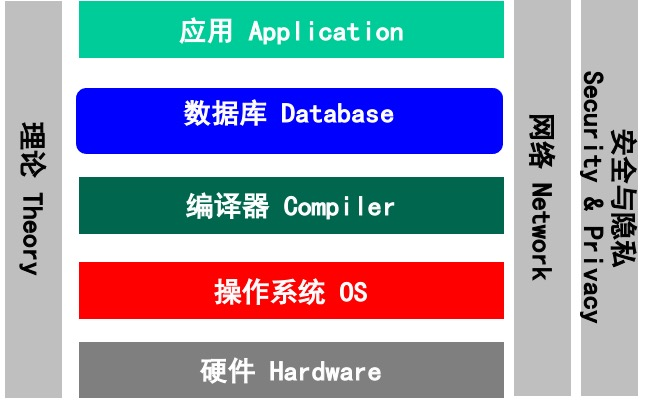
\includegraphics[width=.75\textwidth]{fig23/cs.jpg}
\end{frame}

\begin{frame}
\frametitle{面向AI的计算机系统} 		
\centering	
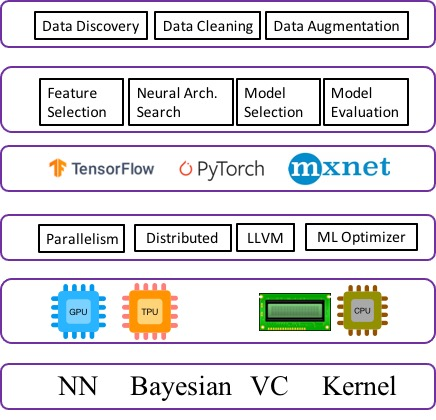
\includegraphics[width=.5\textwidth]{fig23/aios.jpg}
\end{frame}


\begin{frame}
\frametitle{提纲} % Table of contents slide, comment this block out to remove it
\tableofcontents
\end{frame}


\subsection{可大可小,万物互联}

\begin{frame}
\frametitle{可大可小}
\centering	
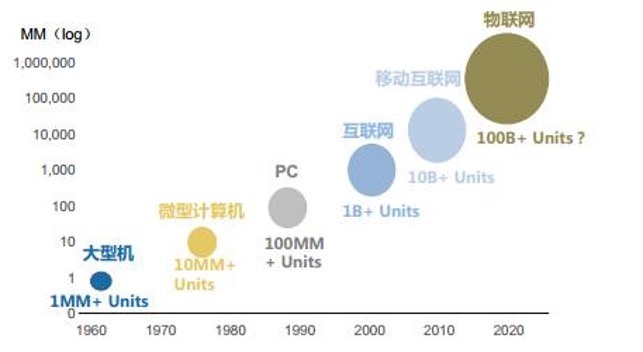
\includegraphics[width=.8\textwidth]{fig23/os.jpg}
\end{frame}


\begin{frame}
\frametitle{万物互联}
\centering	
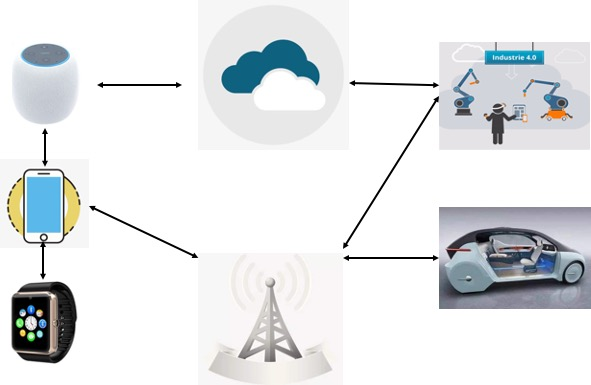
\includegraphics[width=.75\textwidth]{fig23/os2.jpg}
\end{frame}

\begin{frame}
\frametitle{万物互联}
\centering	
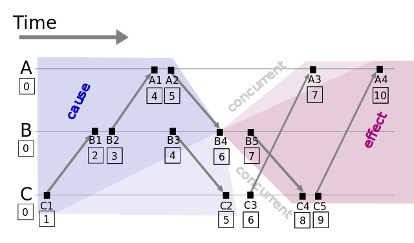
\includegraphics[width=.75\textwidth]{fig23/time.jpg}
\end{frame}



\begin{frame}
\frametitle{异构硬件}
\centering	
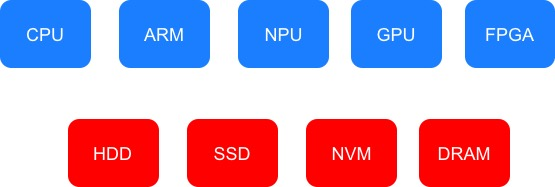
\includegraphics[width=.75\textwidth]{fig23/os3.jpg}
\end{frame}


\begin{frame}
\frametitle{异构硬件通信}
\begin{columns}
		\begin{column}{.55\textwidth}
		\begin{block}{CPU}
			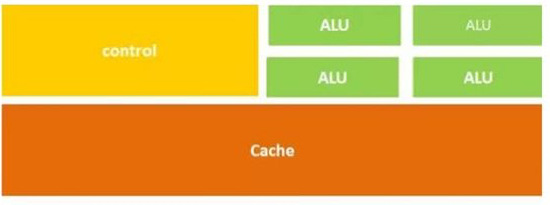
\includegraphics[width=\textwidth]{fig23/cpu.jpg}
		\end{block}
		\end{column}
		\begin{column}{.45\textwidth}
		\begin{block}{GPU}
			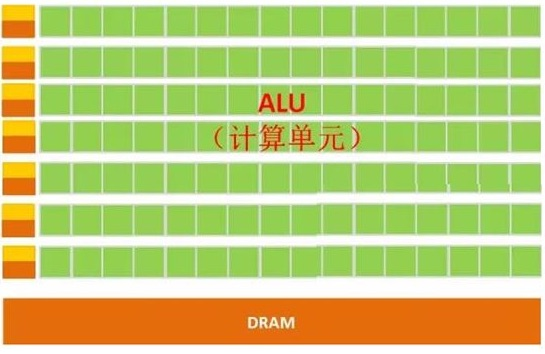
\includegraphics[width=1.\textwidth]{fig23/gpu.jpg}
		\end{block}
		\end{column}
\end{columns}
\end{frame}

\begin{frame}
\frametitle{可大可小,万物互联}
\begin{block}{Motivation}
\begin{itemize}
	\item 不同硬件,同一个系统,一次开发,多次部署
	\item 
		\begin{itemize}
		\item 智能车、耳机、手表、手环、音箱、大屏、家电
	\end{itemize} 
	\item 多端协同,端边云协同,网络化
	\item 可拼装,可插拔(积木化)
	\item 智能硬件
\end{itemize} 
\end{block}
\end{frame}

\begin{frame}
\frametitle{可大可小,万物互联}
\begin{block}{目标}
\begin{itemize}
	\item 分布式
	\item 低时延
	\item 高吞吐
	\item 高可靠
	\item 高弹性伸缩
	\item 多租隔离
\end{itemize} 
\end{block}
\end{frame}


\begin{frame}
\frametitle{可大可小,万物互联}
\begin{block}{云OS}
\begin{itemize}
	\item 虚拟化
	\item 大规模集群资源管理
	\item 分布式文件系统
	\item 资源调度
	\item 安全
\end{itemize} 
\end{block}
\end{frame}


\begin{frame}
\frametitle{可大可小,万物互联}
\begin{block}{Cloud OS}
\centering
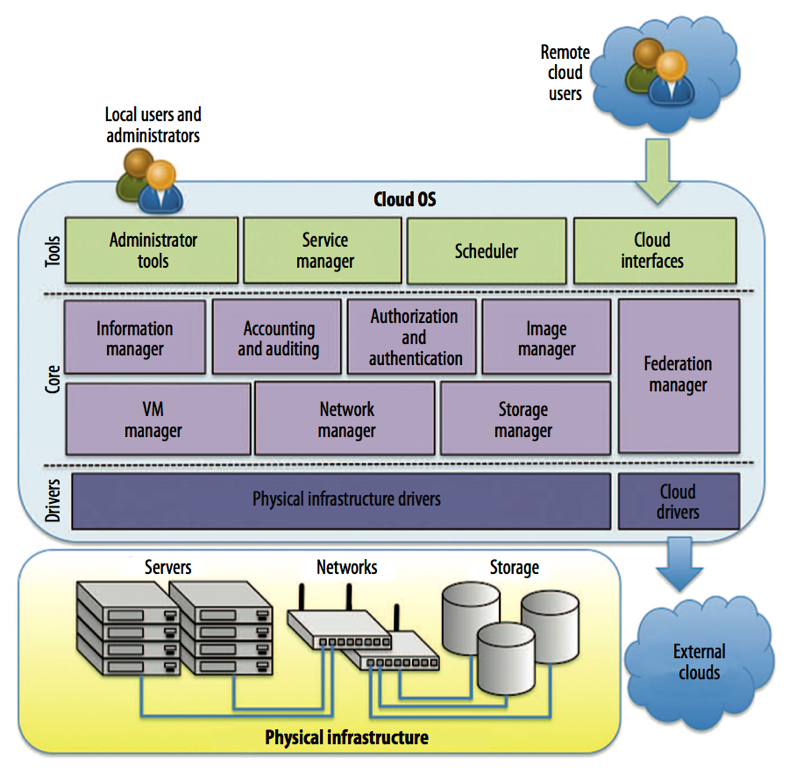
\includegraphics[width=0.5\textwidth]{fig23/cloudos.jpg}
\end{block}
\end{frame}



\begin{frame}
\frametitle{可大可小,万物互联}
\begin{block}{VM vs Docker}
\centering
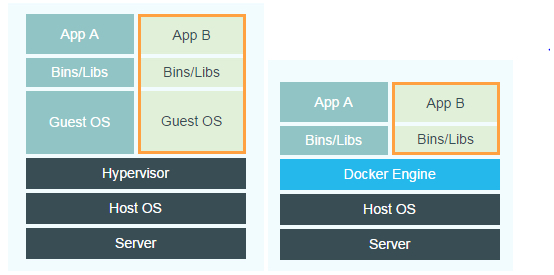
\includegraphics[width=0.8\textwidth]{fig23/docker.jpg}
\end{block}
\end{frame}




\subsection{安全攸关,可信可靠}

\begin{frame}
\frametitle{安全攸关,可信可靠}
\begin{block}{Motivation}
\begin{itemize}
	\item 可控制性
	\item 韧性
	\item 保密、可用、完整
	\item 安全、可追溯
\end{itemize} 
\end{block}
\end{frame}


\begin{frame}
\frametitle{安全攸关,可信可靠}
\begin{block}{CIA}
\begin{itemize}
	\item Confidentiality: Encryption
	\item Integrity: MD5
	\item Availability
\end{itemize} 
\end{block}
\end{frame}





\begin{frame}
\frametitle{安全攸关,可信可靠}
\begin{block}{技术}
\begin{itemize}
	\item 形式化方法
	\item 分层韧性设计
	\item SGX/TEE
	\item Access Control Systems
	\item Authentication Systems
	\item Logging
	\item Filesystem Encryption
	\item Automatic Updates
\end{itemize} 
\end{block}
\end{frame}



\begin{frame}
\frametitle{安全攸关,可信可靠}
\begin{block}{Formal Method}
\centering
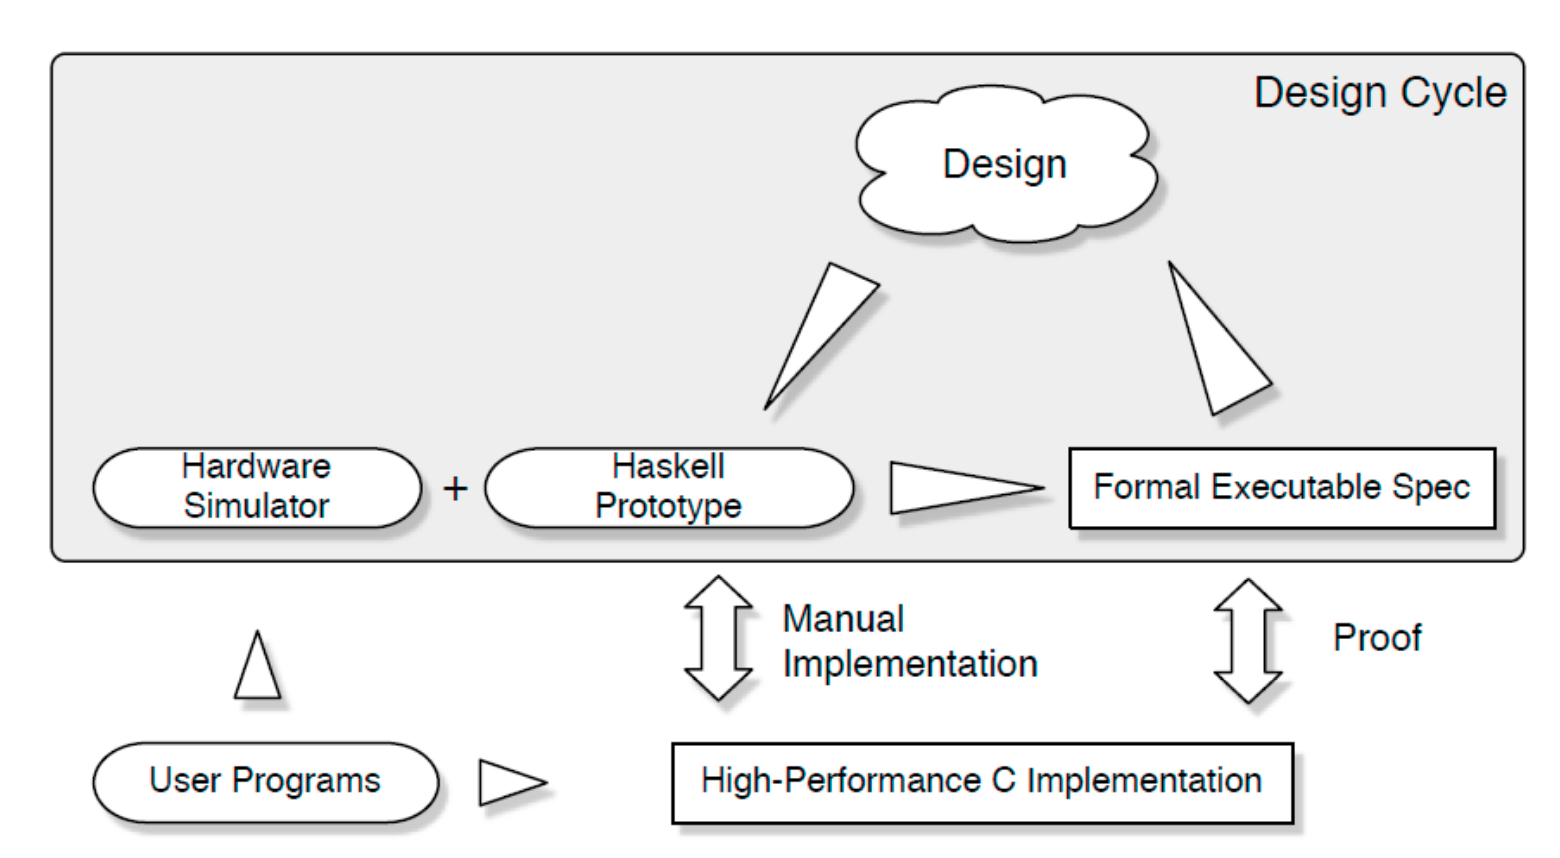
\includegraphics[width=0.6\textwidth]{fig23/formal.jpg}
\end{block}
\end{frame}

\begin{frame}
\frametitle{安全攸关,可信可靠}
\begin{block}{Formal Method}
\centering
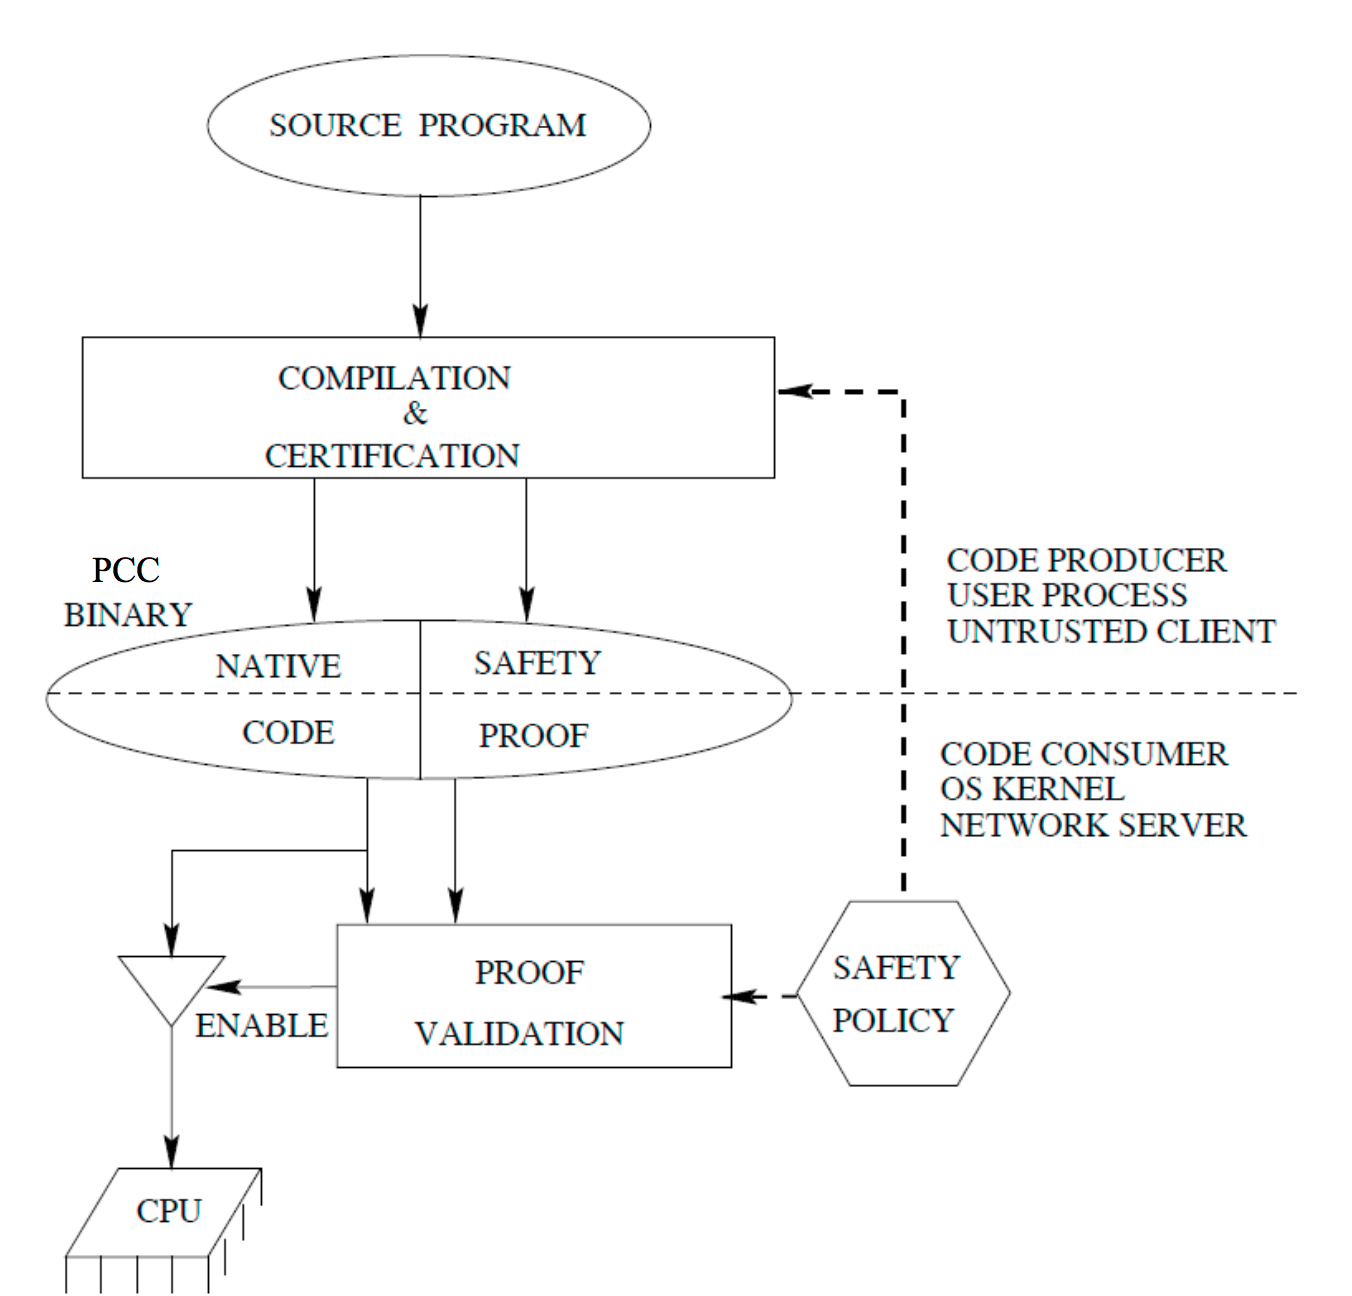
\includegraphics[width=0.5\textwidth]{fig23/formal2.jpg}
\end{block}
\end{frame}

\begin{frame}
\frametitle{安全攸关,可信可靠}
\begin{columns}
		\begin{column}{.455\textwidth}
		\begin{block}{Intel SGX}
			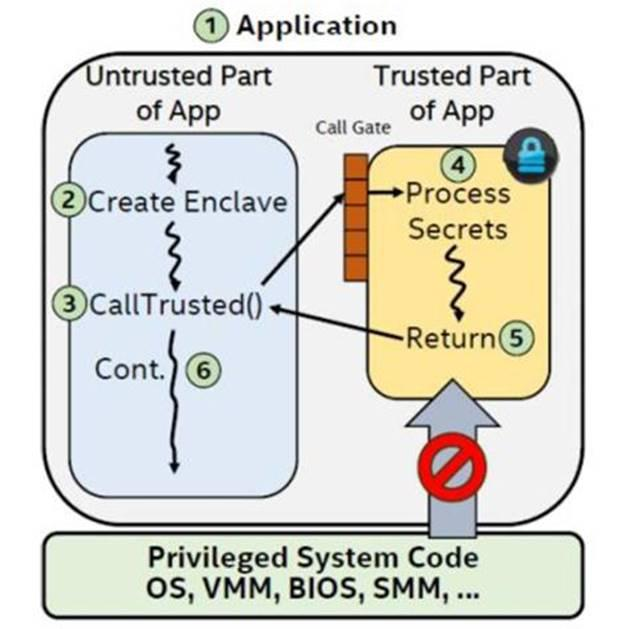
\includegraphics[width=0.84\textwidth]{fig23/sgx.jpeg}
		\end{block}
		\end{column}
		\begin{column}{.55\textwidth}
		\begin{block}{ARM TEE}
			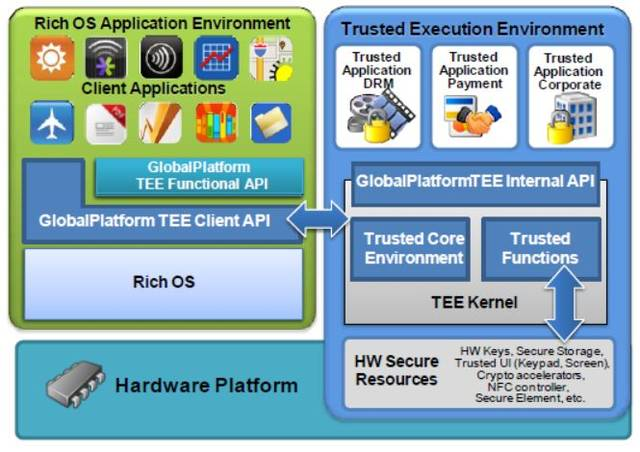
\includegraphics[width=1.\textwidth]{fig23/tee.jpeg}
		\end{block}
		\end{column}
\end{columns}
\end{frame}



\begin{frame}
\frametitle{安全攸关,可信可靠}
\begin{block}{Motivation}
\centering
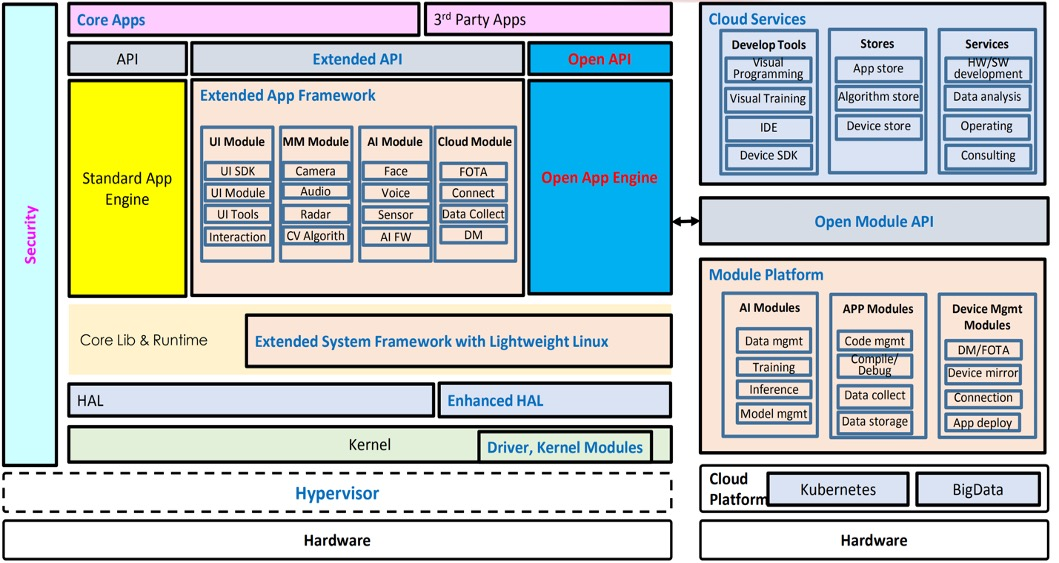
\includegraphics[width=0.8\textwidth]{fig23/os-security.jpg}
\end{block}
\end{frame}


\subsection{以数据为中心}
\begin{frame}
\frametitle{以数据为中心}
\begin{block}{Motivation}
\begin{itemize}
	\item Big Data
	\item Huge number of tasks
	\item Thousands of cores
	\item Network: TCP/IP $\leadsto$ RDMA, programable Nic
	\item States: huge
	\item New hardware: ARM, GPU, NVM, TPU, FPGA
\end{itemize} 
\end{block}
\end{frame}

\begin{frame}
\frametitle{以数据为中心}
\begin{block}{Challenges}
\begin{itemize}
	\item All OS state should be stored in tables in the DBMS.
	\item All changes to OS state should be through DBMS transactions
	\item The DBMS should be leveraged to perform all functions of which it is capable.
\end{itemize} 
\end{block}
\end{frame}


\begin{frame}
\frametitle{以数据为中心}
\begin{block}{Challenges}
\begin{itemize}
	\item Inter-Process Communication
	\item Task Mangement 
	\item File system: file $\leadsto$ table
\end{itemize} 
\end{block}
\end{frame}




\subsubsection{File System}

\begin{frame}
\frametitle{File System}
\begin{block}{Challenges}
\begin{itemize}
	\item Concurrency control 
	\item Crash recovery 
	\item High availability 
	\item Hierarchical block structure 
	\item Scale out
\end{itemize} 
\end{block}
\end{frame}


\begin{frame}
\frametitle{File System}
\begin{block}{Solution: DB transactions}
\begin{itemize}
	\item High speed 
	\item Multiple node 
	\item High availability, crash recovery, concurrency control
	\item Scale out
\end{itemize} 
\end{block}
\end{frame}

\begin{frame}
\frametitle{File System}
\begin{block}{Solution: DB access control}
\begin{itemize}
	\item SQL access control 
	\item Security 
	\item Users, multi-tenants
\end{itemize} 
\end{block}
\end{frame}


\begin{frame}
\frametitle{File System}
\begin{block}{Solution: Complicated Analytics}
\begin{itemize}
	\item Huge number of files
	\item High performance 
	\item Concurrency
	\item Buffer and caching
\end{itemize} 
\end{block}
\end{frame}


\subsubsection{Inter-Process Communication (IPC)}

\begin{frame}
\frametitle{Inter-Process Communication (IPC)}
\begin{block}{Solution: Table Partition and Messaging}
\begin{itemize}
	\item Sender: SQL insert 
	\item Receiver: SQL query
	\item Message ordering and correctness
	\item Semantics
\end{itemize} 
\end{block}
\end{frame}


\begin{frame}
\frametitle{Inter-Process Communication (IPC)}
\begin{block}{Solution: RDMA}
\begin{column}{.5\textwidth}
\begin{itemize}
	\item bypass CPU
	\item low latency, high bandwidth
\end{itemize} 
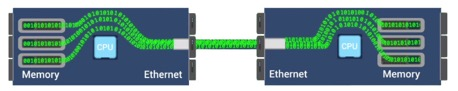
\includegraphics[width=\textwidth]{fig23/rdma0.jpg}
\end{column}
\begin{column}{.5\textwidth}
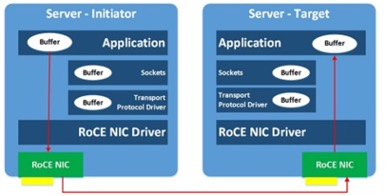
\includegraphics[width=\textwidth]{fig23/rdma2.jpg}
\end{column}
\end{block}
\end{frame}


\begin{frame}
\frametitle{Inter-Process Communication (IPC)}
\begin{block}{Solution: RDMA}
\begin{column}{.5\textwidth}
\begin{itemize}
	\item High elastic 
	\item high resource utilization
	\item high availability 
	\item Heterogenous hardware
\end{itemize} 
\end{column}
\begin{column}{.5\textwidth}
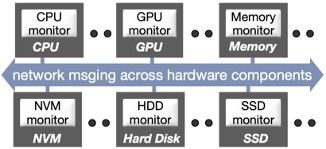
\includegraphics[width=0.8\textwidth]{fig23/rdma3.jpg}
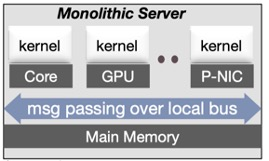
\includegraphics[width=0.8\textwidth]{fig23/rdma4.jpg}
\end{column}
\end{block}
\end{frame}


\begin{frame}
\frametitle{Inter-Process Communication (IPC)}
\begin{block}{Solution: Shared Memory}
\begin{column}{.5\textwidth}
\begin{itemize}
	\item Memory sharing
	\item cloud computing 
	\item Activate-Passive Replication
	\item Activate-Activate Replication
\end{itemize} 
\end{column}
\begin{column}{.5\textwidth}
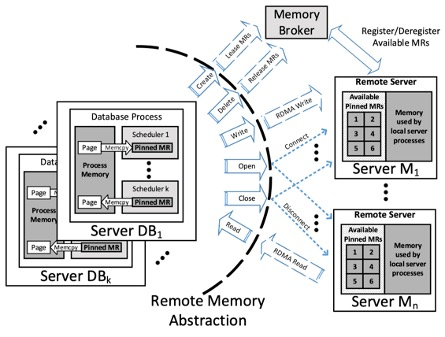
\includegraphics[width=\textwidth]{fig23/rdma5.jpg}
\end{column}
\end{block}
\end{frame}


\subsubsection{Task Management}

\begin{frame}
\frametitle{Task Management}
\begin{block}{Solution: Global Table Scheduling}
\begin{itemize}
	\item Partitioned tables
	\item Table scheduling  
	\item Global scheduling
	\item Scheduler is a query (with user-defined function)
\end{itemize} 
\end{block}
\end{frame}



\begin{frame}
\frametitle{Task Management}
\begin{block}{Solution: Straggler}
\begin{itemize}
	\item Query scheduling 
	\item SMP
	\item Massive parallel
	\item Analytics
\end{itemize} 
\end{block}
\end{frame}






\begin{frame}
\frametitle{Task Management}
\begin{block}{SMP}
\begin{column}{.5\textwidth}

\begin{itemize}
	\item Symmetric Multi-Processor (SMP)
	\item Uniform Memory Access
	\item Full parallel
	\item Processors with local caches
\end{itemize} 

\end{column}
\begin{column}{.5\textwidth}
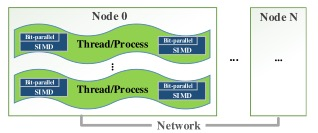
\includegraphics[width=\textwidth]{fig23/smp.jpg}
\end{column}

\end{block}
\end{frame}


\begin{frame}
\frametitle{Task Management}
\begin{block}{SMP: Cache Coherence}
\begin{column}{.5\textwidth}

\begin{itemize}
	\item Managing replication and migration of data between CPUs
	\item The unit of replication and consistency is the cache line
	\item false sharing 
\end{itemize} 

\end{column}
\begin{column}{.5\textwidth}
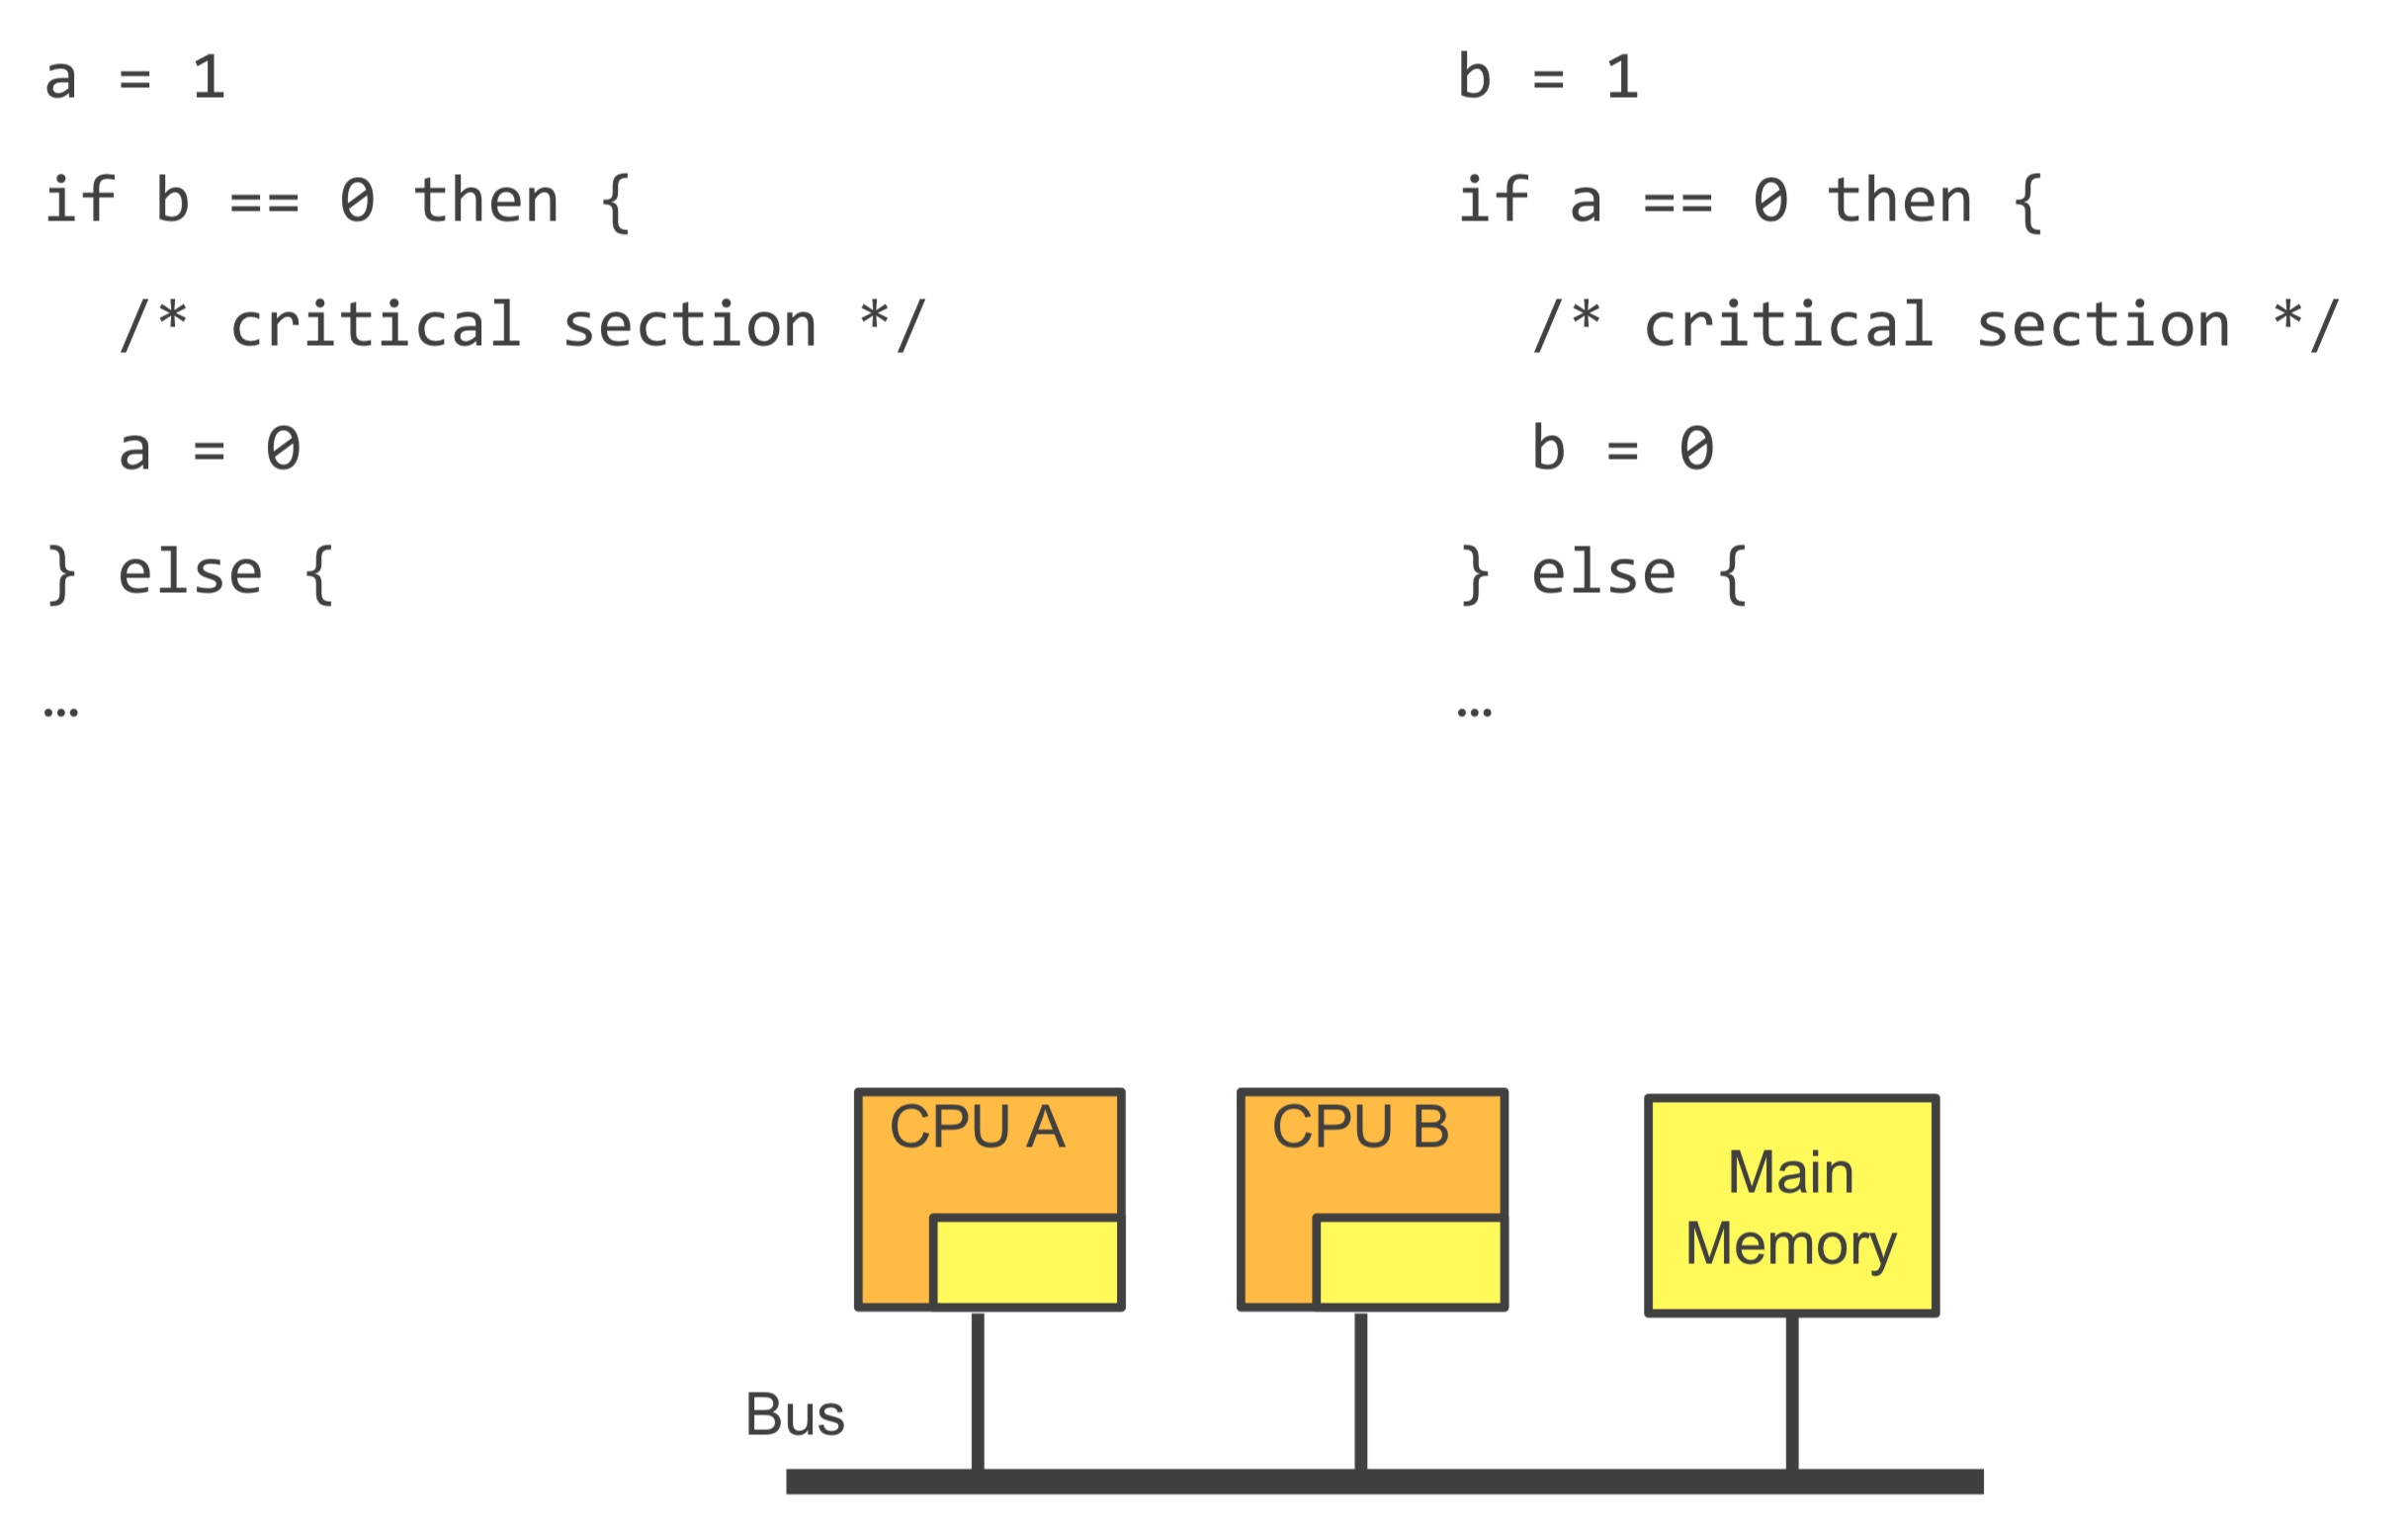
\includegraphics[width=\textwidth]{fig23/smp2.jpg}
\end{column}

\end{block}
\end{frame}







\begin{frame}
\frametitle{Task Management}
\begin{block}{ARM}
\begin{column}{.5\textwidth}

\begin{itemize}
	\item ARM
	\item NUMA
\end{itemize} 

\end{column}
\begin{column}{.5\textwidth}
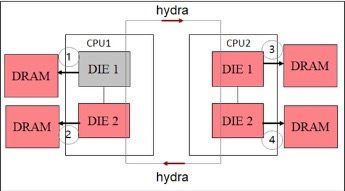
\includegraphics[width=\textwidth]{fig23/numa.jpg}
\end{column}

\end{block}
\end{frame}

\begin{frame}
\frametitle{Task Management}
\begin{block}{CPU + GPU}
\begin{column}{.5\textwidth}

\begin{itemize}
	\item UDF on hardware 
	\item Function as a service
	\item Hardware-software co-design
\end{itemize} 

\end{column}
\begin{column}{.5\textwidth}
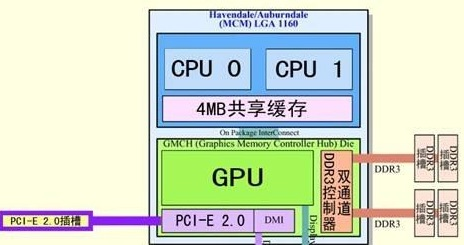
\includegraphics[width=\textwidth]{fig23/cpugpu.jpg}
\end{column}

\end{block}
\end{frame}



\begin{frame}
\frametitle{Task Management}
\begin{block}{NVM}
\begin{column}{.5\textwidth}

\begin{itemize}
	\item NVM
	\item Byte Addressable 
	\item Non-Volatile
	\item High speed
\end{itemize} 

\end{column}
\begin{column}{.5\textwidth}
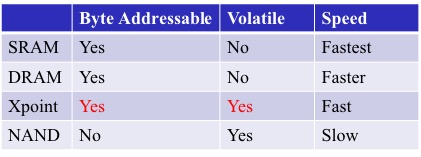
\includegraphics[width=\textwidth]{fig23/nvm.jpg}
\end{column}

\centering
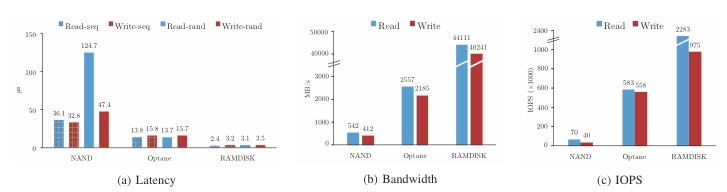
\includegraphics[width=0.8\textwidth]{fig23/nvm2.jpg}
\end{block}
\end{frame}

\subsubsection{Provenance}

\begin{frame}
\frametitle{Provenance}
\begin{block}{Motivation}
\begin{itemize}
	\item Who update my salary?
	\item Who change my picture and what she has changed?
	\item Is an image changed?
\end{itemize} 
\end{block}
\end{frame}





\begin{frame}
\frametitle{Provenance}
\begin{block}{Solution}
\begin{itemize}
	\item Data debugging
	\item Data consumption and understanding
	\item Tamper Proof
	\item Non-repudiation
	\item Backtracking 
	\item Logging
\end{itemize} 
\end{block}
\end{frame}




\begin{frame}
\frametitle{以数据为中心}
\begin{block}{Advantages}
\begin{itemize}
	\item Performance optimization
	\item Security
	\item Virtualization and containerization
	\item Geographic distributability
	\item More sophisticated file management
	\item Better scheduling
	\item Enhanced state management
\end{itemize} 
\end{block}
\end{frame}









\begin{frame}
\frametitle{OS Research}
\begin{block}{Research topics}
\begin{itemize}
	\item Integration with programming languages and runtimes
	\item Concurrent/parallel programming models; scheduling
	\item Security and virtualization
	\item Networking, storage, and distributed systems
	\item Tracing and debugging techniques
	\item Formal modeling and verification
	\item As a platform for other research – e.g., mobile systems
\end{itemize} 
\end{block}
\end{frame}










\iffalse
%\begin{frame}
%\frametitle{提纲} % Table of contents slide, comment this block out to remove it
%\tableofcontents % Throughout your presentation, if you choose to use \section{} and \subsection{} commands, these will automatically be printed on this slide as an overview of your presentation
%\end{frame}
%
%%----------------------------------------------------------------------------------------
%%	PRESENTATION SLIDES
%%----------------------------------------------------------------------------------------
%
%%------------------------------------------------
%\section{第一节:课程概述} % Sections can be created in order to organize your presentation into discrete blocks, all sections and subsections are automatically printed in the table of contents as an overview of the talk
%%------------------------------------------------
%-------------------------------------------------
\begin{frame}[plain]
	\frametitle{Introduction}
	
	
	
	\begin{columns}
		
		\begin{column}{.4\textwidth}
			
			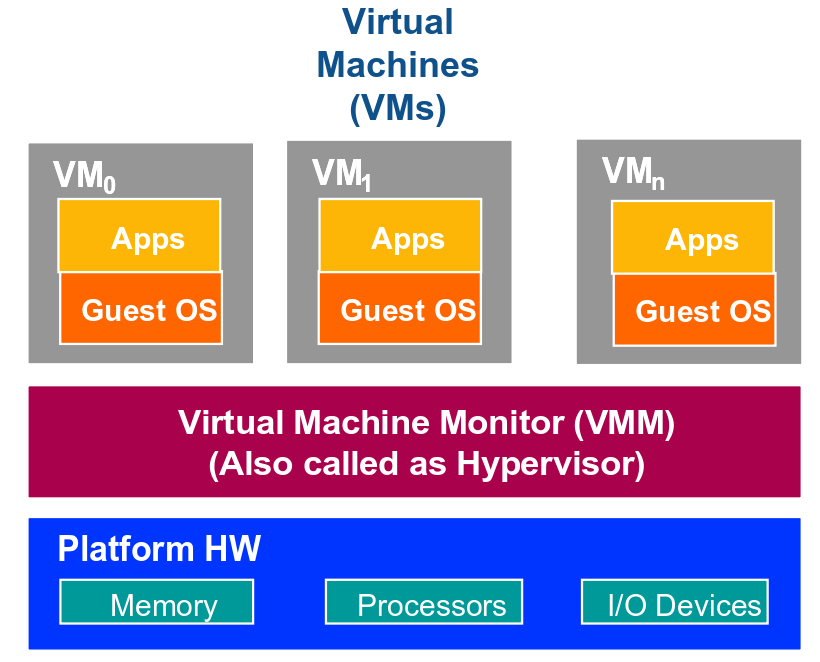
\includegraphics[width=1.\textwidth]{vmm-overview}
			
		\end{column}
		
		\begin{column}{.6\textwidth}
			
		
			\begin{block}{What is Virtualization}
				Virtualization is a term that refers to the abstraction of computer resources [wikipedia]
			\end{block}
		
			\begin{block}{Wisdom}
				All computer problems can be solved with another layer of redirection [Donald E. Knuth (高德纳), Stanford University]
			\end{block}

		\end{column}
		
		
	\end{columns}
	
	
\end{frame}

%-------------------------------------------------
\begin{frame}[plain]
	\frametitle{Introduction -- taxonomy}



	\begin{columns}

	\begin{column}{.3\textwidth}
	
	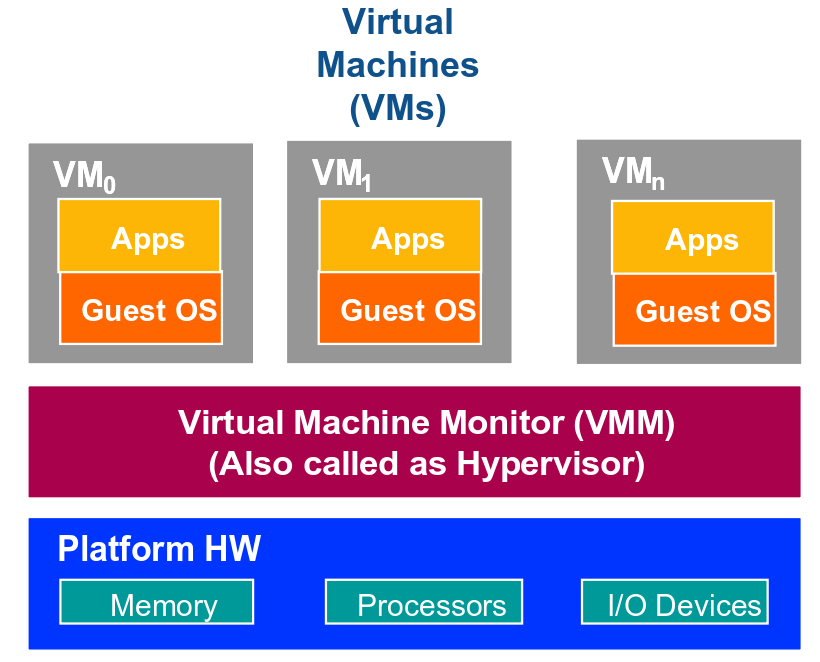
\includegraphics[width=1.\textwidth]{vmm-overview}
	
	\end{column}

	\begin{column}{.7\textwidth}
	
%	\Large
%    OS Structure	
%	\begin{itemize}
%	\item Simple kernel
%%	\item Monolithic kernel
%%	\item Micro kernel
%%	\item Exokernel
%%	\item VMM, etc...
%	\end{itemize}	

	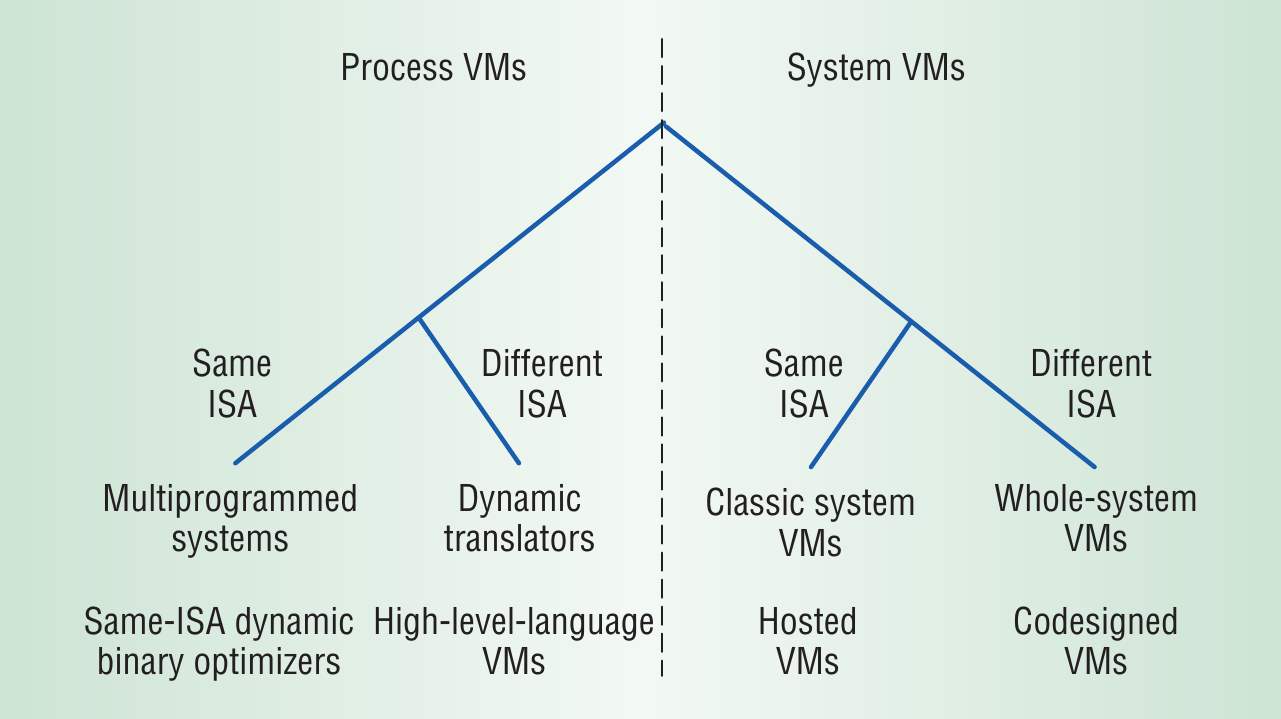
\includegraphics[width=1.\textwidth]{vm-taxonomy}
	
	\tiny	
	from James E.Smith,     IEEE computer Society2005	
	\end{column}
	
    
\end{columns}


\end{frame}

%-------------------------------------------------
\begin{frame}[plain]
	\frametitle{Introduction -- different layer of virtualization}
	
	
	
	\begin{columns}
		
		\begin{column}{.3\textwidth}
			
			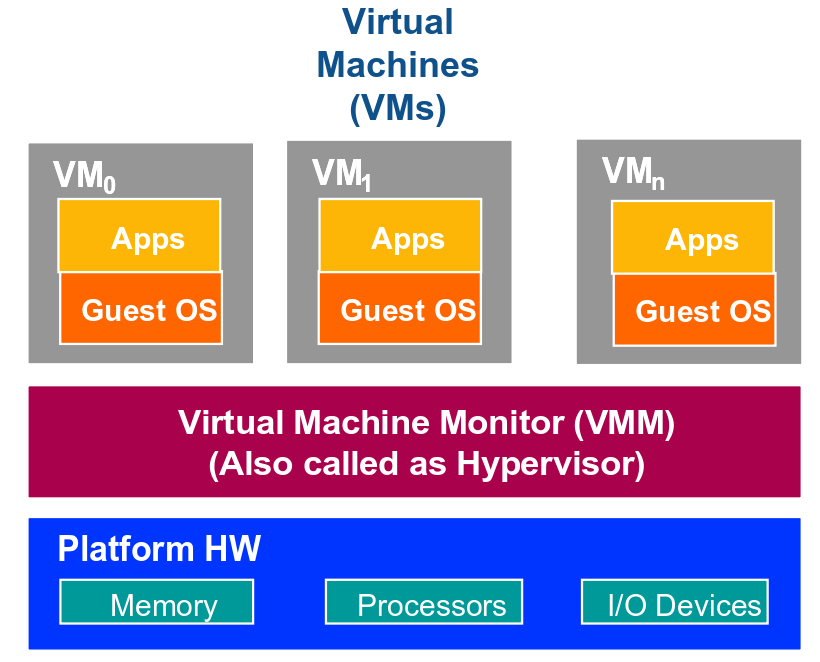
\includegraphics[width=1.\textwidth]{vmm-overview}
			
		\end{column}
		
		\begin{column}{.5\textwidth}
			
			%	\Large
			%    OS Structure	
			%	\begin{itemize}
			%	\item Simple kernel
			%%	\item Monolithic kernel
			%%	\item Micro kernel
			%%	\item Exokernel
			%%	\item VMM, etc...
			%	\end{itemize}	
			
			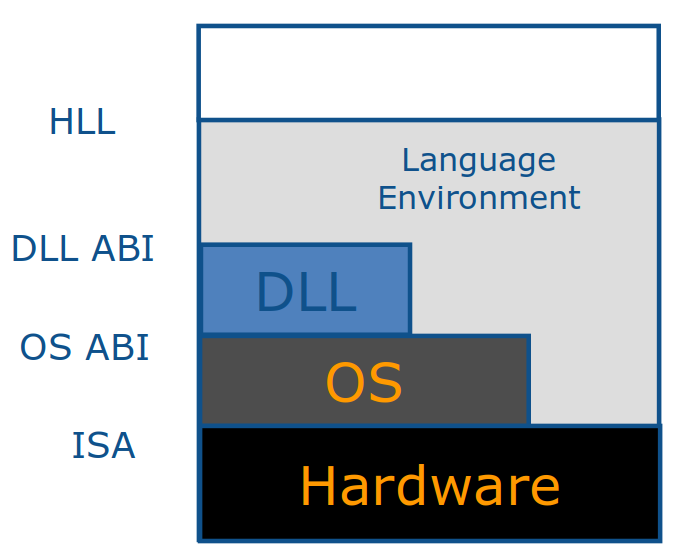
\includegraphics[width=1.\textwidth]{vm-layer}
			
			
		\end{column}
		
		
	\end{columns}
	
	
\end{frame}


%-------------------------------------------------
\begin{frame}[plain]
	\frametitle{Introduction -- VMM}
	
	
	
	\begin{columns}
		
		\begin{column}{.5\textwidth}
			
			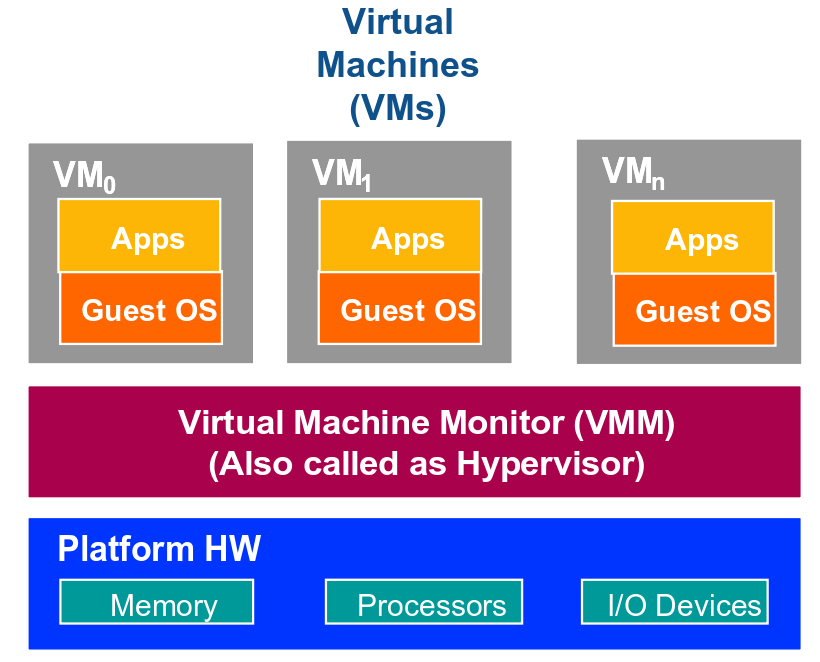
\includegraphics[width=1.\textwidth]{vmm-overview}
			
		\end{column}
		
		\begin{column}{.5\textwidth}
			
			\begin{block}{Virtual Machine Monitor, VMM}
	VMM transforms the single machine interface into the illusion of many. Each of these interfaces (virtual machines) is an efficient replica of the original computer system, complete with all of the processor instructions [Robert P. Goldberg, 1974]
			\end{block}
			
%			\begin{block}{Virtual Machine Monitor, VMM}
%				A virtual machine is implemented by adding software to an execution platform to give it the appearance of a different platform, or for that matter, to give the appearance of multiple platforms. [. E. Smith and Ravi Nair, “An Overview of Virtual Machine Architectures”.]
%			\end{block}
		\end{column}
		
		
	\end{columns}
	
	
\end{frame}

%-------------------------------------------------
\begin{frame}[plain]
	\frametitle{Introduction -- VMM}
	
	
	
	\begin{columns}
		
		\begin{column}{.5\textwidth}
			
			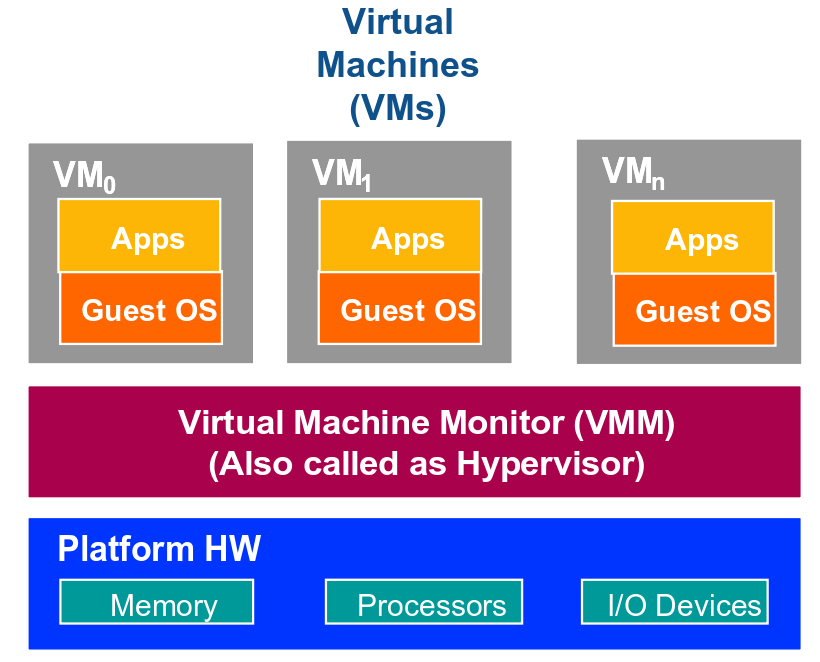
\includegraphics[width=1.\textwidth]{vmm-overview}
			
		\end{column}
		
		\begin{column}{.5\textwidth}
			
%			\begin{block}{Virtual Machine Monitor, VMM}
%				VMM transforms the single machine interface into the illusion of many. Each of these interfaces (virtual machines) is an efficient replica of the original computer system, complete with all of the processor instructions [Robert P. Goldberg, 1974]
%			\end{block}
			
			\begin{block}{Virtual Machine Monitor, VMM}
				A virtual machine is implemented by adding software to an execution platform to give it the appearance of a different platform, or for that matter, to give the appearance of multiple platforms. [J.E. Smith, “An Overview of Virtual Machine Architectures”]
			\end{block}
		\end{column}
		
		
	\end{columns}
	
	
\end{frame}


%-------------------------------------------------
\begin{frame}[plain]
	\frametitle{Introduction -- Why VMM?}
	
	
	
	\begin{columns}
		
		\begin{column}{.5\textwidth}
			
			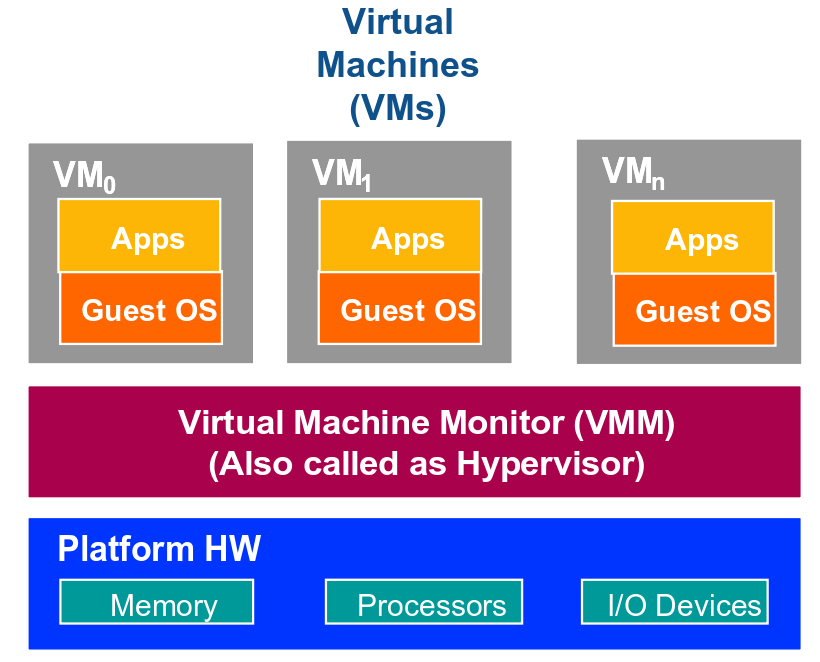
\includegraphics[width=1.\textwidth]{vmm-overview}
			
		\end{column}
		
		\begin{column}{.5\textwidth}
		
		Before there were data centers... 
		\begin{itemize}
			\item Many early commercial computers were mainframes
			\item powerful computation, highly reliable, extensive I/O capabilities
			\item for computing/data-intensive  apps 
			
		\end{itemize} 	
        IBM	System/360 hardware and CP/CMS system software: Virtualizable Architecture
		\end{column}
		
		
	\end{columns}
		
\end{frame}


%-------------------------------------------------
\begin{frame}[plain]
	\frametitle{Introduction -- Why VMM?}
	
	
	
	\begin{columns}
		
		\begin{column}{.5\textwidth}
			
			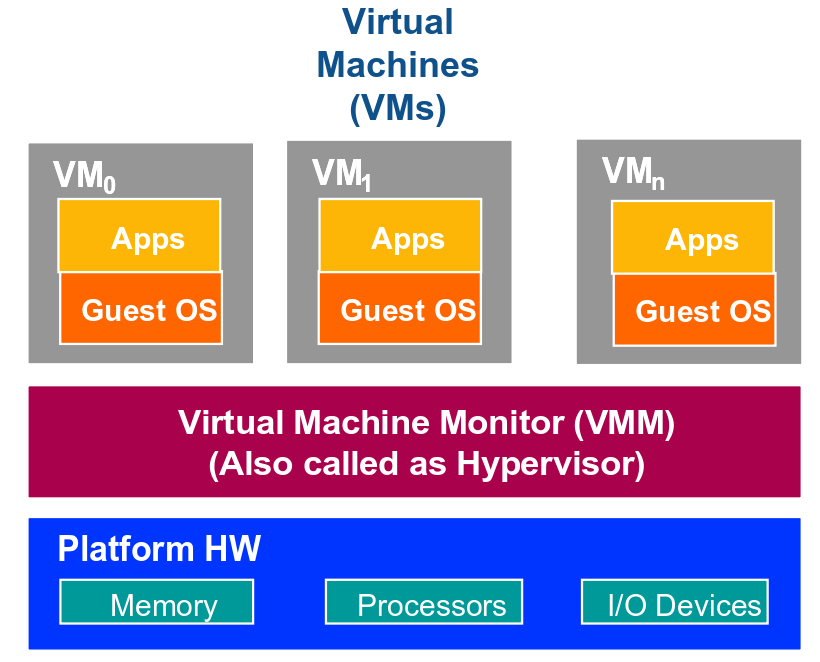
\includegraphics[width=1.\textwidth]{vmm-overview}
			
		\end{column}
		
		\begin{column}{.5\textwidth}
			
			Now there were data centers... 
			\begin{itemize}
				\item Many computers were servers connected in the world.
				\item powerful computation, highly reliable, extensive I/O capabilities
				\item for computing/data-intensive apps 

				
			\end{itemize} 	
			 x86/ARM and Linux/KVM, vmware, xen, etc. system software: Virtualizable Architecture
		\end{column}
		
		
	\end{columns}
	
\end{frame}


%-------------------------------------------------
\begin{frame}[plain]
	\frametitle{Introduction -- Essential characteristics of VMM}
	
	
	
	\begin{columns}
		
		\begin{column}{.5\textwidth}
			
			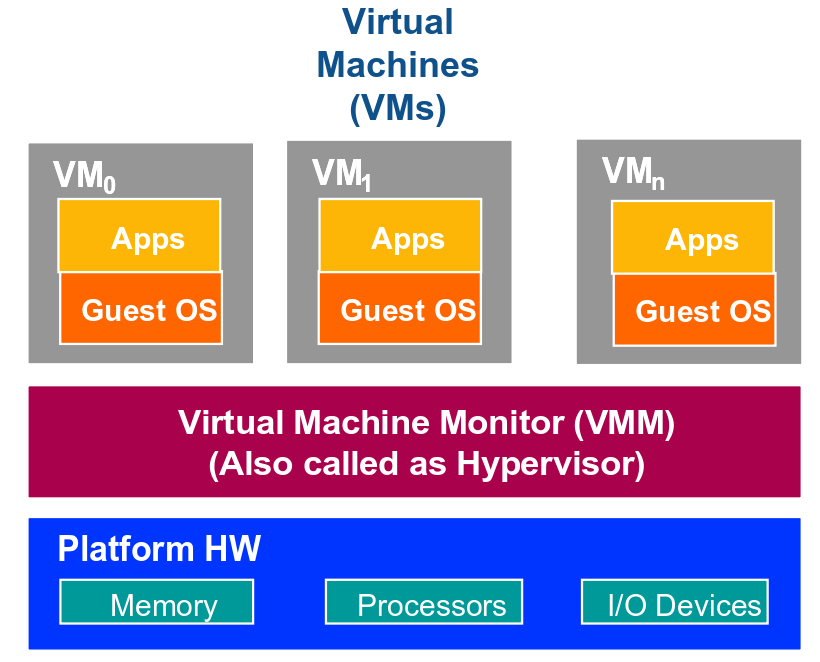
\includegraphics[width=1.\textwidth]{vmm-overview}
			
		\end{column}
		
		\begin{column}{.5\textwidth}
			
	     \begin{itemize}
			\item Equivalence: Essentially identical virtual platform, except
			\begin{itemize}
				\item Differences caused by the availability of system resources. e.g. memory size

			\end{itemize} \pause
			
			\item Isolation, or resource control 
			\begin{itemize}
				\item VMM is in complete control of system resources
				
			\end{itemize} \pause
			
			\item Efficiency
			\begin{itemize}
				\item At worst only minor decreases in speed
				\item speed $>>$ emulators, software interpreters (simulators)
				
			\end{itemize}
		
     	\end{itemize}	
	
		\end{column}
		
		
	\end{columns}
	
	
\end{frame}

\fi
%-------------------------------------------------


\end{document}